\section{Results}
\label{sec:results}

\subsection{Observed price paths}
\label{sec:paths}

Figure~\ref{fig:paths} shows each chip's realized price path relative to its first observed
six-month bin, holding provider, region, contract and the other controls fixed. These paths need
no identification assumption. The older chips decline slowly and unevenly: the V100 changes by
\nPathVHundredFour{} log points over four years and \nPathVHundredNine{} over nine, and the A100
40GB reaches \nPathAHundredFive{} at five years. The H100's rent instead rose in its first year
(\nPathHHundredOne), fell to \nPathHHundredThree{} at three years, and recovered to
\nPathHHundredFour{} at four years in the 2026 shortage. \ajcheck{Realized paths are not smooth
decays. They are long flat stretches, sharp falls and demand-driven rebounds, and the 2026 shortage
reverses part of the decline for every chip still on sale.}

\begin{figure}[htbp]
\centering
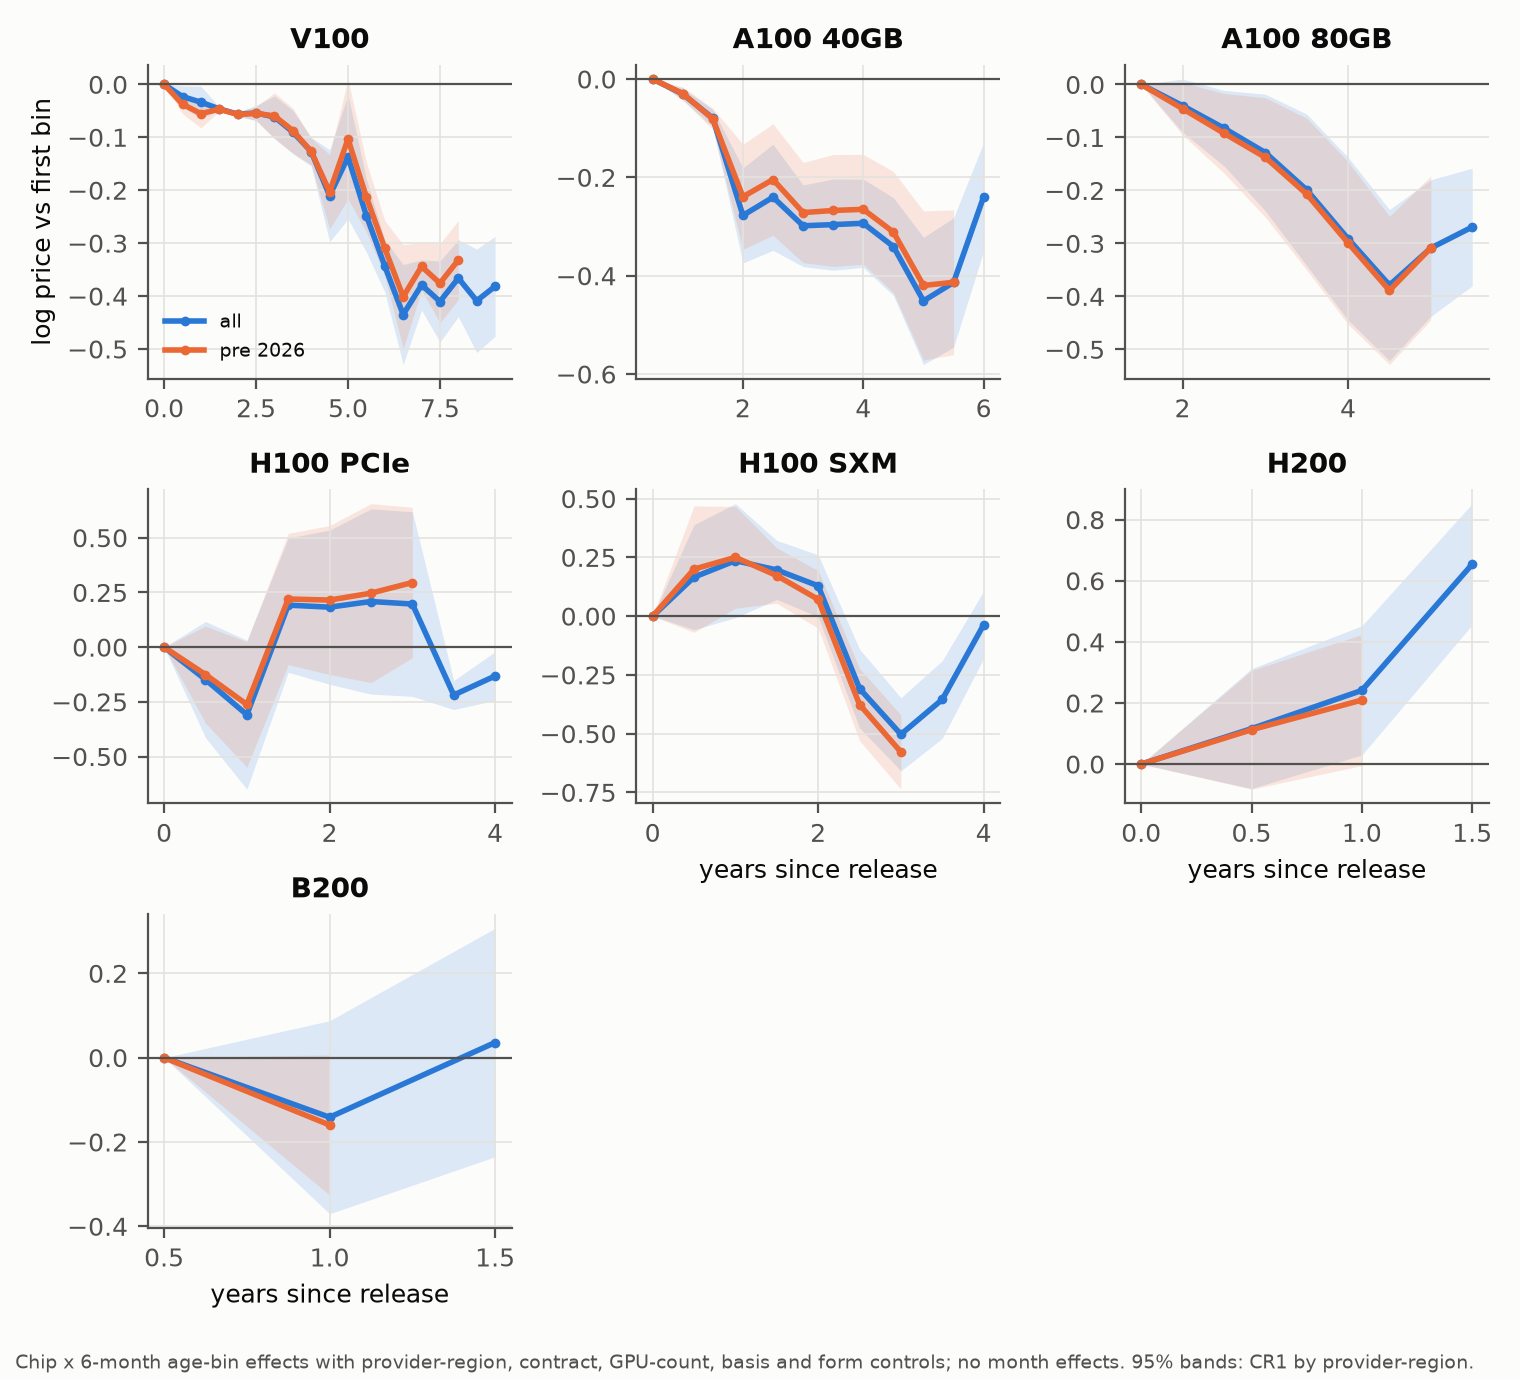
\includegraphics[width=0.85\textwidth]{p5a_cohort_paths.png}
\caption{Observed cohort paths: log real price by six-month age bin relative to each chip's first
bin, with provider $\times$ region, contract $\times$ term, GPU count, price basis and form-factor
controls and no month effects. Bands: 95\% intervals, CR1 by provider-region.}
\label{fig:paths}
\end{figure}

\subsection{Age profiles under four identification strategies}
\label{sec:profiles}

Table~\ref{tab:strategies} and Figure~\ref{fig:profiles} report the strategies that identify a
linear term, and the shape-only strategy. Strategy 1 prices each log point of TFLOP/s at
\nTflopsCoef{} log points of rent. It finds no decline with age over the first two years (rate
\nOneARateEarly, interval [\nOneARateEarlyLo, \nOneARateEarlyHi]) and roughly none after
(\nOneARateLate). Strategy 2's age profile rises slightly and then falls (\nTwoRateEarly{} and
\nTwoRateLate{} a year). Strategy 4's shape estimate is \nFourShape{}
[\nFourShapeLo, \nFourShapeHi] under the pre-registered bootstrap. Every point estimate of the
early minus late rate is positive: prices fall later, not earlier, against H1.

\begin{table}[htbp]
\centering
\caption{Summary of the age profile by identification strategy (full sample)}
\label{tab:strategies}
\begin{adjustbox}{max width=\textwidth}
% Generated by gel.viz.hedonic_figures from p5_summary.csv. Do not edit.
\begin{tabular}{lccccc}
\hline
Strategy & $g(2)-g(0)$ & $g(4)-g(0)$ & rate, yrs 0--2 & rate, yrs 2--4 & early $-$ late rate (H1: $<0$) \\
\hline
1a quality index (TFLOP/s) & 0.55 [-0.45, 1.55] & 0.48 [-0.06, 1.03] & 0.27 [-0.23, 0.77] & -0.03 [-0.24, 0.18] & 0.31 [-0.52, 1.11] \\
1b three specs & 0.55 [-0.57, 1.68] & 0.55 [-0.61, 1.69] & 0.28 [-0.28, 0.84] & -0.00 [-0.50, 0.47] & 0.28 [-0.42, 0.97] \\
2 frontier-relative & 0.22 [-0.25, 0.69] & -0.08 [-0.77, 0.62] & 0.11 [-0.12, 0.35] & -0.15 [-0.41, 0.11] & 0.26 [0.05, 0.47] \\
4 shape only & -- & -- & -- & -- & 0.47 [0.36, 0.57] \\
\hline
\end{tabular}

\end{adjustbox}
\par\smallskip\footnotesize Log points; rates are per year. Brackets: 95\% intervals from the
unrestricted wild cluster bootstrap at the chip level (7 clusters, Webb weights, 9,999 draws). These
intervals are too narrow; see Table~\ref{tab:review}.
\end{table}

\begin{figure}[htbp]
\centering
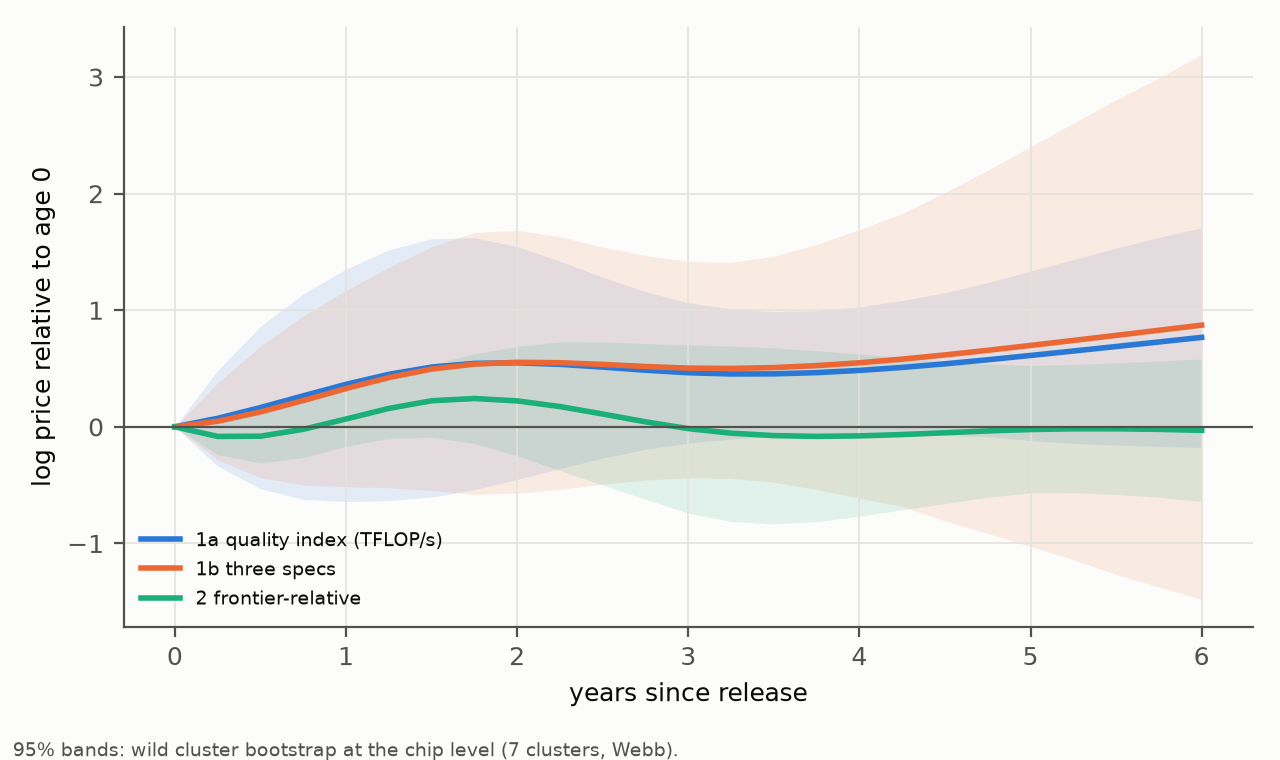
\includegraphics[width=0.49\textwidth]{p5b_strategy_profiles.png}
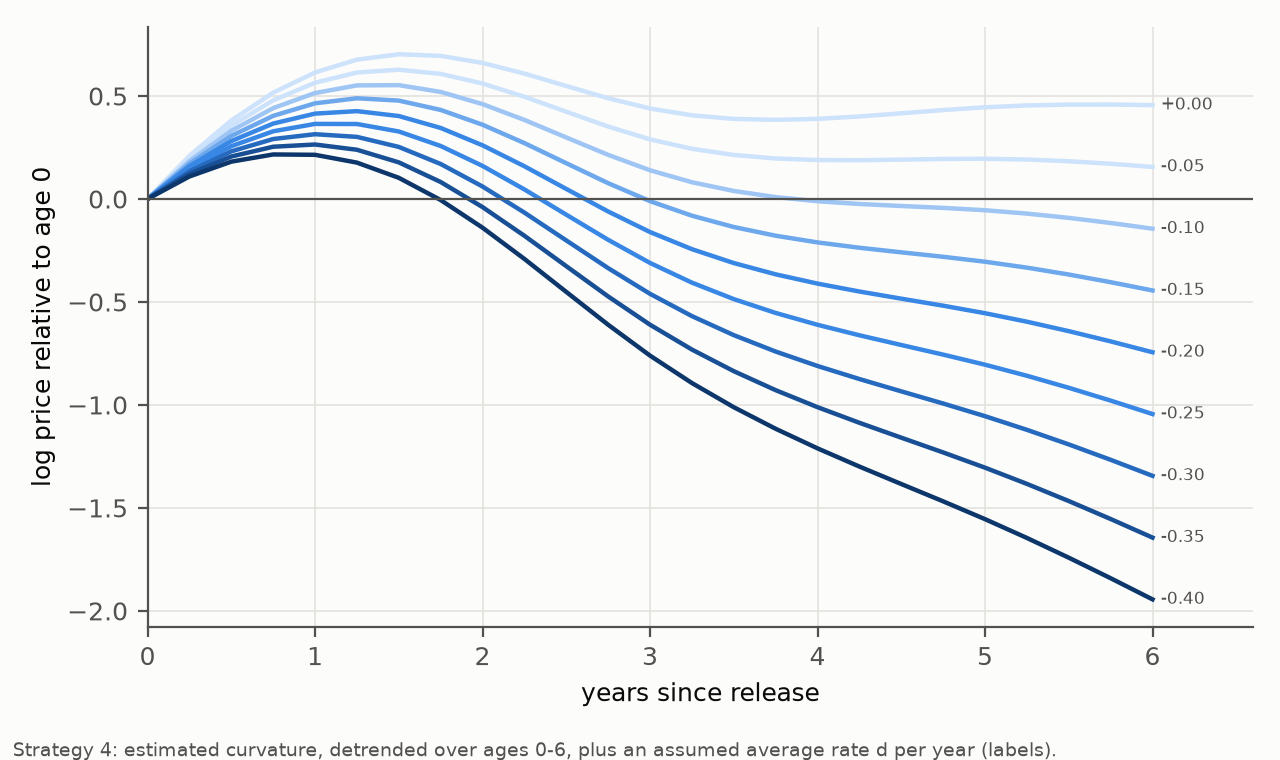
\includegraphics[width=0.49\textwidth]{p5c_strategy4_sweep.png}
\caption{Age profiles $g(a) - g(0)$ under strategies 1a, 1b and 2 (left) and strategy 4 for
assumed average rates $d$ from 0 to $-0.40$ log points a year (right).}
\label{fig:profiles}
\end{figure}

\subsection{What survives valid inference}
\label{sec:review}

An adversarial review of these results, written by a reader with no access to the author's notes,
identified three problems; Table~\ref{tab:review} and the checks below address them.

\emph{The intervals are too narrow.} In a Monte Carlo that keeps this panel's rows, fixed effects
and regressors and draws errors with the estimated residual structure under a true shape of zero,
the unrestricted bootstrap's 95\% intervals cover the truth \nCovWcuLo--\nCovWcuHi{} of the time
and CR1 by chip \nCovCrchipLo--\nCovCrchipHi{} (\nMcReps{} replications per design); the restricted
bootstrap covers \nCovWcrLo--\nCovWcrHi. Under the restricted bootstrap no summary measure is
significant: strategy 4's shape has $p = \nFourShapeWcrP$ (unrestricted $p$ \nFourShapeWcuP) and
a test-inversion interval of [\nFourShapeWcrLo, \nFourShapeWcrHi], and strategy 2's has
$p = \nTwoShapeWcrP$.

\emph{The shape is identified only from vintage-specific trends.} Allowing each chip its own
linear calendar trend leaves the quadratic term unidentified; at a zero quadratic term the shape is
\nShapeChipTrendZero. Reassigning release dates across chips, the actual assignment gives the
largest shape of \nPermAssignments{} distinct assignments ($p = \nPermP$), so the curvature is tied
to release order. \ajcheck{That test cannot tell an age effect from demand trends that are
themselves ordered by vintage, such as the 2023--26 shortages that hit the newest chips.}

\emph{The answer depends on the market.} The shape is \nFourShapeSpot{} for spot prices
[\nFourShapeSpotLo, \nFourShapeSpotHi] and \nFourShapeOnDemand{} for on-demand prices
[\nFourShapeOnDemandLo, \nFourShapeOnDemandHi]. Restricting to the \nListMoversRows{} non-spot
listings whose price changes at least once, it is \nShapeListMovers{} (provider-clustered standard
error \nShapeListMoversSe), in H1's direction. Weighting providers equally cuts the pooled shape to
\nShapeEqualProv.

\begin{table}[htbp]
\centering
\caption{Unrestricted (WCU) and restricted (WCR) wild cluster bootstrap $p$-values}
\label{tab:review}
% Generated by gel.viz.paper_numbers from p5_review_wcr.csv.
\begin{tabular}{llrrrr}
\hline
Strategy & Measure & Estimate & SE (CR1, chip) & $p$ (WCU) & $p$ (WCR) \\
\hline
1a quality index & rate, yrs 0--2 & 0.27 & 0.16 & 0.300 & 0.649 \\
1a quality index & rate, yrs 2--4 & $-$0.03 & 0.06 & 0.615 & 0.678 \\
1a quality index & early $-$ late & 0.31 & 0.19 & 0.421 & 0.735 \\
1b three specs & rate, yrs 0--2 & 0.28 & 0.16 & 0.262 & 0.595 \\
1b three specs & rate, yrs 2--4 & 0.00 & 0.14 & 0.991 & 0.993 \\
1b three specs & early $-$ late & 0.28 & 0.22 & 0.591 & 0.820 \\
2 frontier-relative & rate, yrs 0--2 & 0.11 & 0.09 & 0.297 & 0.494 \\
2 frontier-relative & rate, yrs 2--4 & $-$0.15 & 0.06 & 0.208 & 0.228 \\
2 frontier-relative & early $-$ late & 0.26 & 0.10 & 0.006 & 0.305 \\
4 shape only & early $-$ late & 0.47 & 0.08 & $<$0.0001 & 0.287 \\
\hline
\end{tabular}

\par\smallskip\footnotesize Null: measure $= 0$. Chip-level clusters (7), Webb weights, 9,999
draws. SE: CR1 clustered by chip.
\end{table}

\ajcheck{Taken together, the projection strategies do not establish either the speed or the shape
of the age profile in this sample. The observed cohort paths are the more credible guide to the
rate, and the dependence of the shape on the market read is itself a finding.}

\subsection{Successor releases}
\label{sec:events}

Figure~\ref{fig:events} shows the predecessor's price around its successor's release. There is no
detectable drop: prices in the first year after release are \nHTwo{} [\nHTwoLo, \nHTwoHi] relative
to the six months before. The one negative bin, \nEvSixEleven{} at 6--11 months, falls where cloud
availability of the successor actually began; dating events by the successor's first listing in
the panel moves that bin earlier, and neither dating detects a drop (H2).

\begin{figure}[htbp]
\centering
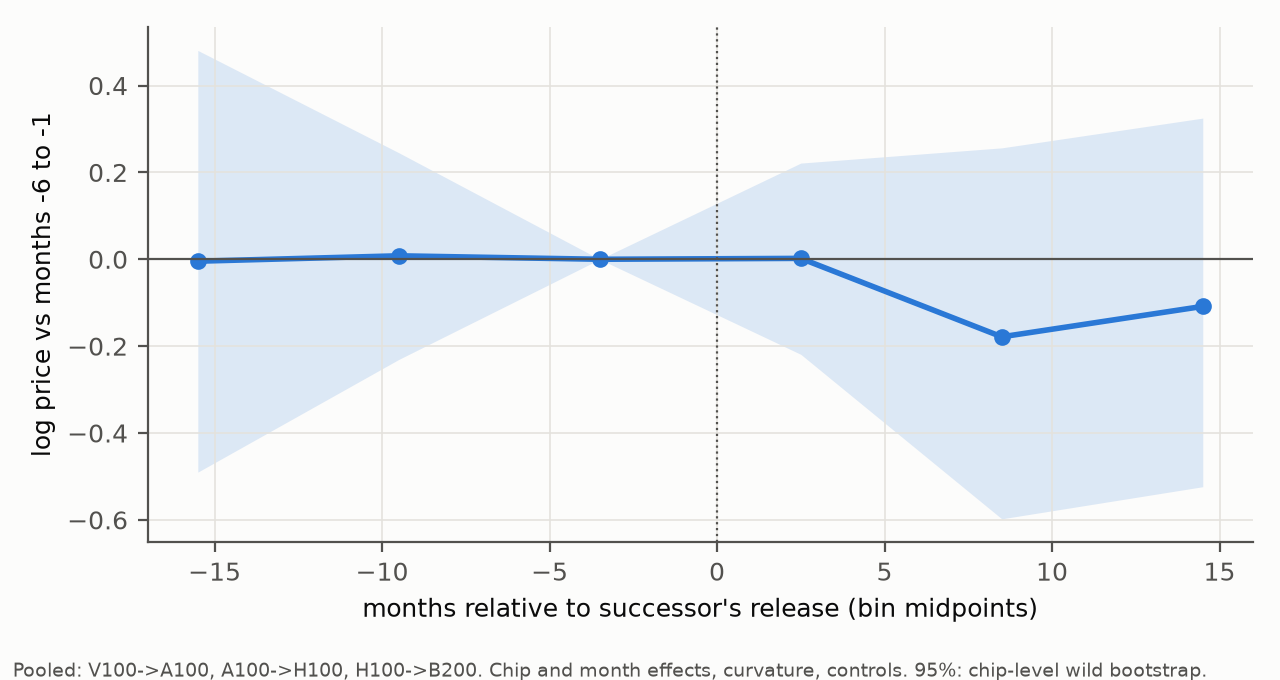
\includegraphics[width=0.6\textwidth]{p5d_event_study.png}
\caption{Successor event study: predecessor prices by six-month event-time bin around the
successor's Epoch release month, relative to months $-6$ to $-1$; chip and month effects and
controls. Bands: unrestricted chip-level bootstrap.}
\label{fig:events}
\end{figure}

\subsection{Asset values and economic life}
\label{sec:values}

Table~\ref{tab:values} and Figure~\ref{fig:values} turn the rent paths into values. Along the
realized path an H100 loses \nValRealLostOne{} of its value in the first year and
\nValRealLostThree{} by year three, and its straight-line-equivalent life is \nValRealSle{} years:
value declines more slowly than under any five- or six-year straight-line schedule. Strategy 2 gives
a similar curve (\nValTwoLostThree{} by year three). Only an assumed average decline of
0.40 log points a year in strategy 4 produces a front-loaded curve (\nValFourFortyLostThree{} lost by
year three, life \nValFourFortySle{} years), and it implies a launch rent of \$\nValFourFortyRentZero{}
an hour for the H100, far above any rent in the panel.

\begin{table}[htbp]
\centering
\caption{Asset values and straight-line-equivalent lives}
\label{tab:values}
\begin{adjustbox}{max width=\textwidth}
% Generated by gel.models.asset_value from p6_summary.csv. Do not edit.
% Base case r = 10%, u = 70%, PUE 1.3, system power, 2%/yr failure; brackets: min-max over the r x u x PUE grid.
\begin{tabular}{llcccc}
\hline
Chip & Rent path & $V(0)$/capex & Share lost by yr 3 & SL-equivalent life (yrs) & $T^*$ (yrs) \\
\hline
A100 80GB & Realized (V100, A100) & 5.32 [3.41, 7.48] & 0.32 [0.31, 0.33] & 9.4 [9.2, 9.6] & $>$9 \\
A100 80GB & 2 frontier-relative & 4.83 [3.07, 6.83] & 0.28 [0.27, 0.30] & 10.1 [9.8, 10.3] & $>$9 \\
A100 80GB & 4 shape, d = -0.20 & 9.08 [6.02, 12.48] & 0.52 [0.52, 0.53] & 7.2 [7.0, 7.3] & $>$9 \\
A100 80GB & 4 shape, d = -0.40 & 19.94 [13.58, 26.82] & 0.71 [0.71, 0.72] & 5.0 [4.9, 5.1] & $>$9 \\
H100 SXM & Realized (V100, A100) & 4.49 [2.89, 6.31] & 0.32 [0.31, 0.33] & 9.4 [9.2, 9.6] & $>$9 \\
H100 SXM & 2 frontier-relative & 4.55 [2.91, 6.41] & 0.28 [0.27, 0.30] & 10.1 [9.9, 10.3] & $>$9 \\
H100 SXM & 4 shape, d = -0.20 & 5.89 [3.87, 8.11] & 0.53 [0.52, 0.54] & 7.1 [6.9, 7.3] & $>$9 \\
H100 SXM & 4 shape, d = -0.40 & 8.89 [6.00, 12.02] & 0.72 [0.72, 0.74] & 4.9 [4.8, 5.0] & $>$9 \\
H200 & Realized (V100, A100) & 5.57 [3.60, 7.80] & 0.32 [0.31, 0.33] & 9.4 [9.2, 9.6] & $>$9 \\
H200 & 2 frontier-relative & 4.81 [3.08, 6.79] & 0.28 [0.27, 0.30] & 10.1 [9.9, 10.3] & $>$9 \\
H200 & 4 shape, d = -0.20 & 4.00 [2.58, 5.57] & 0.54 [0.53, 0.56] & 7.0 [6.7, 7.2] & $>$9 \\
H200 & 4 shape, d = -0.40 & 3.81 [2.49, 5.23] & 0.76 [0.74, 0.79] & 4.5 [4.1, 4.7] & $>$9 \\
B200 & Realized (V100, A100) & 4.45 [2.87, 6.23] & 0.32 [0.31, 0.33] & 9.4 [9.2, 9.6] & $>$9 \\
B200 & 2 frontier-relative & 3.84 [2.45, 5.42] & 0.28 [0.27, 0.30] & 10.1 [9.8, 10.3] & $>$9 \\
B200 & 4 shape, d = -0.20 & 3.18 [2.05, 4.44] & 0.54 [0.53, 0.57] & 7.0 [6.7, 7.1] & $>$9 \\
B200 & 4 shape, d = -0.40 & 3.03 [1.97, 4.17] & 0.76 [0.75, 0.80] & 4.4 [4.0, 4.7] & $>$9 \\
\hline
\end{tabular}

\end{adjustbox}
\par\smallskip\footnotesize $V(0)$/capex: value at release over capital cost. SL-equivalent life:
$2\int_0^H V(a)/V(0)\,da$. $T^*$: first age at which utilization $\times$ rent $\le$ operating cost.
Operating cost excludes hosting, network and staff, so $V(0)$/capex is an upper bound.
\end{table}

\begin{figure}[htbp]
\centering
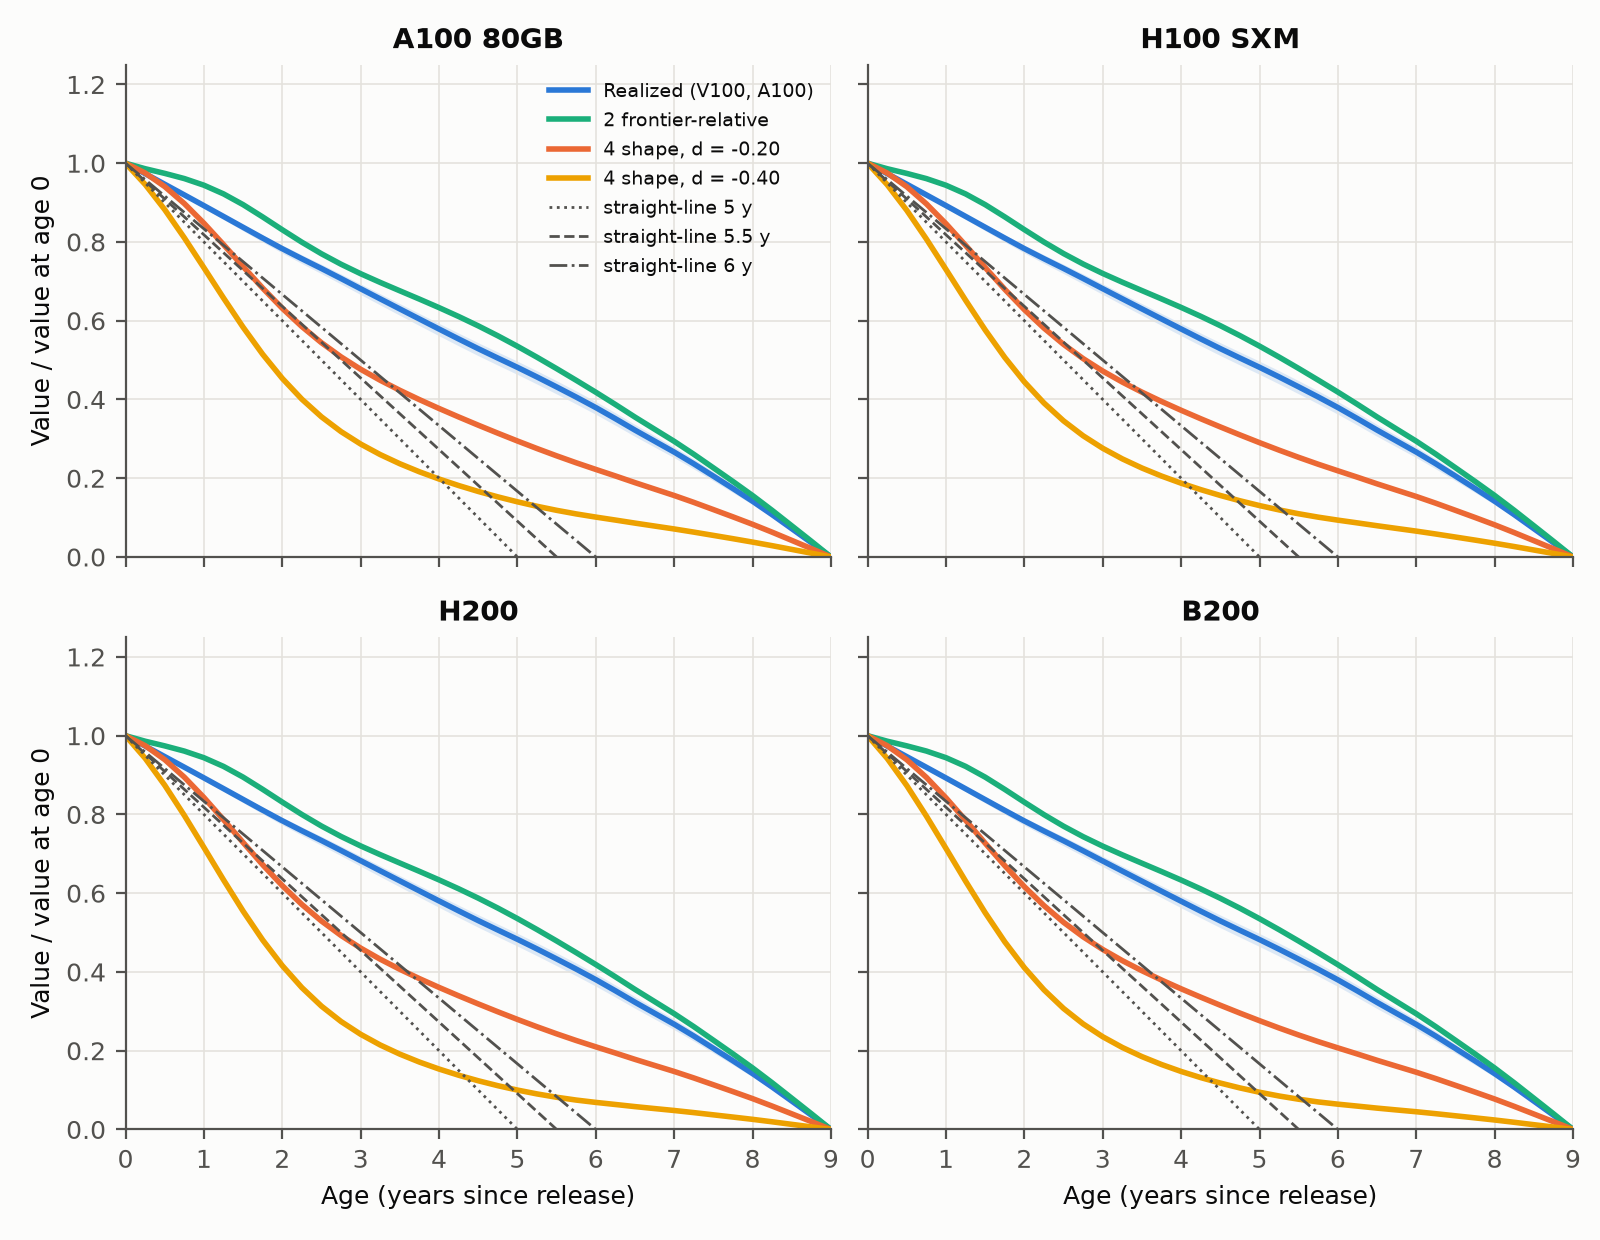
\includegraphics[width=0.85\textwidth]{p6_value_curves.png}
\caption{Value relative to value at release, by rent path, against 5-, 5.5- and 6-year
straight-line schedules. Band: the $r \times u \times$ PUE grid around the realized path.}
\label{fig:values}
\end{figure}

Two features of these numbers matter more than their levels. First, $T^*$ \nTstarAll{} binds within
the nine-year horizon: the H100's neocloud rent of \$\nValRentNow{} an hour is many times its
\$\nValOpex{} of power and maintenance, so the end of the value curve is set by the horizon, not by
rents reaching operating cost. With a six-year horizon the straight-line-equivalent life is
\nValRealSleSix{} years, and with five years \nValRealSleFive. \ajcheck{Rents alone do not pin down
economic life; the retirement decision does.} Second, $V(0)$ is \nValRealVzeroLo--\nValRealVzeroHi{}
times capital cost across the grid, which reflects scarcity rents and the omitted hosting costs, so
the value-to-cost ratio should not be read as profitability.

\subsection{Triangulation with benchmark, term-structure and retirement evidence}
\label{sec:triangulation}

A companion analysis measures three other quantities for the same chips: a throughput benchmark
priced at neocloud rents (P1), the decay implied by reserved-to-on-demand price ratios (P2), and a
power-constrained retirement model in which an old chip is replaced when a newer one would earn
more in the same power slot (P3). Table~\ref{tab:triangulation} and Figure~\ref{fig:triangulation}
compare them. Old chips are priced close to their output today (the H100's obsolescence discount
against the H200 is \nPOneDHHundred). Life to operating cost is long: \nPTwoLopexLo--\nPTwoLopexHi{}
years for the H100 from the term structure. In the power-constrained model the median retirement
age is \nPThreeMedian{} years (P10--P90 \nPThreePTen--\nPThreePNinety), rising to
\nPThreeAbundant{} years when power is abundant and \nPThreeNoScarcity{} without a scarcity markup;
about \nMarkupShare{} of today's rent is markup at the calibrated level. \ajcheck{Book lives of four
to six years sit between the power-constrained and the unconstrained answers, close to the
constrained one.}

\begin{table}[htbp]
\centering
\caption{Triangulation of economic life by method}
\label{tab:triangulation}
\begin{adjustbox}{max width=\textwidth}
% Generated by gel.viz.paper_numbers from m8_triangulation.csv.
\begin{tabular}{lrrrr}
\hline
Generation (age, yrs) & P1 discount $D$ & P1 life to opex & P2 life to opex & P3 retirement age (P10--P90) \\
\hline
A100 80GB (6.0) & 0.00 [$-$0.21, 0.20] & 19.9--25.9 & 10.7--13.2 & 4.1 (2.2--7.0) \\
H100 SXM (4.1) & $-$0.02 [$-$0.13, 0.34] & 15.1--20.4 & 9.8--11.7 & 4.1 (2.2--7.0) \\
H200 SXM (2.0) & 0.00 [0.00, 0.00] & 14.3--18.8 & 6.5--7.5 & 4.1 (2.2--7.0) \\
\hline
\end{tabular}

\end{adjustbox}
\par\smallskip\footnotesize P1: obsolescence discount against the H200 at concurrency 32 (median
neocloud price; provider range) and implied life to operating cost. P2: life to operating cost over
the discount-rate and term-premium grid. P3: median retirement age, power-constrained base case.
All lives in years since release.
\end{table}

\begin{figure}[htbp]
\centering
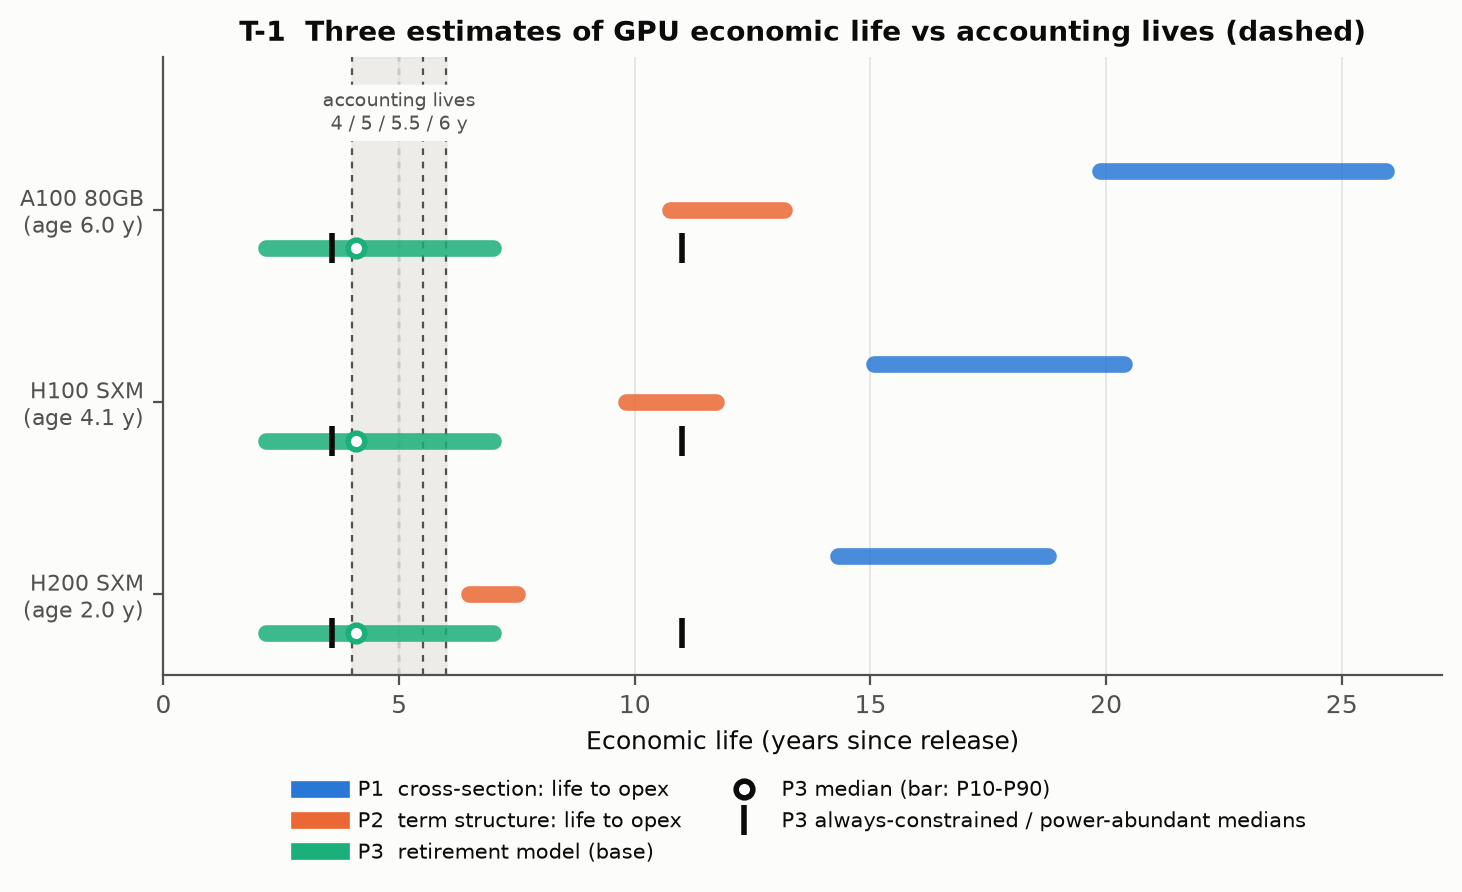
\includegraphics[width=0.75\textwidth]{t1_triangulation.png}
\caption{Economic life by method against accounting lives of 4, 5, 5.5 and 6 years.}
\label{fig:triangulation}
\end{figure}
